%% ============================================================================
%% EVNet Sentinel — Computer Networks Report
%% Subject: Computer Networks
%% Academic Year: 2026–2027
%% ============================================================================
\documentclass[11pt, a4paper]{article}

% ---- Packages ----
\usepackage[utf8]{inputenc}
\usepackage[T1]{fontenc}
\usepackage{lmodern}
\usepackage{microtype}
\usepackage[margin=0.75in]{geometry}
\usepackage{graphicx}
\graphicspath{{images/}{figures/}{./}}
\usepackage{adjustbox}
\usepackage{xcolor}
\usepackage{booktabs}
\usepackage{longtable}
\usepackage{tabularx}
\usepackage{multirow}
\usepackage{enumitem}
\usepackage{hyperref}
\usepackage{fancyhdr}
\usepackage{titlesec}
\usepackage{tcolorbox}
\usepackage{pifont}
\usepackage{array}
\usepackage{caption}
\usepackage{subcaption}
\usepackage{float}

% ---- Colors (shared palette with other project documents) ----
\definecolor{primary}{HTML}{1E40AF}
\definecolor{accent}{HTML}{10B981}
\definecolor{secondary}{HTML}{0D9488}
\definecolor{warning}{HTML}{F59E0B}
\definecolor{danger}{HTML}{EF4444}
\definecolor{darkbg}{HTML}{1F2937}
\definecolor{lightgray}{HTML}{F3F4F6}
\definecolor{sectionblue}{HTML}{2563EB}
\definecolor{lightbg}{HTML}{F8FAFC}

% ---- Hyperref Setup ----
\hypersetup{
    colorlinks=true,
    linkcolor=primary,
    urlcolor=sectionblue,
    citecolor=accent,
    pdftitle={EVNet Sentinel — Computer Networks Report},
    pdfauthor={Group 1 — Vidyalankar Institute of Technology},
    pdfsubject={Computer Networks Academic Report},
    pdfkeywords={IDS, EVCS, Network Security, CICEVSE2024, DoS, Reconnaissance, OCPP, ISO 15118},
    bookmarks=true,
    bookmarksopen=true,
    bookmarksnumbered=true,
}

% ---- Header / Footer ----
\pagestyle{fancy}
\fancyhf{}
\fancyhead[L]{\small\textcolor{primary}{\textbf{EVNet Sentinel}}}
\fancyhead[R]{\small\textcolor{darkbg}{Computer Networks Report}}
\fancyfoot[C]{\thepage}
\renewcommand{\headrulewidth}{0.8pt}
\renewcommand{\footrulewidth}{0.4pt}

% ---- Section Formatting ----
\titleformat{\section}
  {\Large\bfseries\color{primary}}
  {\thesection.}{0.5em}{}[\vspace{-0.3em}\textcolor{accent}{\rule{\textwidth}{1.5pt}}]
\titleformat{\subsection}
  {\large\bfseries\color{sectionblue}}
  {\thesubsection}{0.5em}{}

% ---- tcolorbox styles ----
\newtcolorbox{highlightbox}[1][]{
    colback=primary!5, colframe=primary!70, arc=4pt,
    boxrule=0.8pt, left=8pt, right=8pt, top=6pt, bottom=6pt, #1
}
\newtcolorbox{findingbox}[1][]{
    colback=danger!5, colframe=danger!70, arc=4pt,
    boxrule=0.8pt, left=8pt, right=8pt, top=6pt, bottom=6pt, #1
}
\newtcolorbox{resultbox}[1][]{
    colback=accent!5, colframe=accent!70, arc=4pt,
    boxrule=0.8pt, left=8pt, right=8pt, top=6pt, bottom=6pt, #1
}

% ---- Screenshot placeholder command ----
\newcommand{\screenshotplaceholder}[2]{%
    \begin{figure}[H]
        \centering
        \fcolorbox{primary!40}{lightgray}{%
            \parbox{0.85\textwidth}{%
                \vspace{2.5cm}
                \centering\large\textcolor{darkbg}{\textit{[Screenshot: #1]}}
                \vspace{2.5cm}
            }%
        }
        \caption{#2}
    \end{figure}
}

% ============================================================================
% DOCUMENT START
% ============================================================================
\begin{document}

% ============================================================================
% TITLE PAGE
% ============================================================================
\begin{titlepage}
    \centering
    \vspace*{1cm}

    {\Huge \bfseries Computer Networks\\[0.3cm] Project Report\par}
    \vspace{0.5cm}
    {\large on\par}
    \vspace{0.5cm}

    {\Huge \bfseries\textcolor{primary}{EVNet Sentinel}\par}
    \vspace{0.2cm}
    {\Large\textit{Network Intrusion Detection for\\Electric Vehicle Charging Infrastructure}\par}

    \vspace{1.2cm}

    \begin{tcolorbox}[colback=lightbg, colframe=primary!50, arc=6pt, boxrule=0.6pt, width=0.75\textwidth]
        \centering
        {\large \textbf{Subject:} Computer Networks}\\[0.2cm]
        {\large \textbf{Academic Year:} 2026--2027}
    \end{tcolorbox}

    \vspace{1cm}

    {\Large \bfseries Prepared by: Group 1\par}
    \vspace{0.5cm}
    {\large
    \begin{tabular}{|c|l|l|}
        \hline
        \textbf{Roll No.} & \textbf{Name} & \textbf{Role} \\ \hline
        24102A0013 & Mukta Varak & Cloud Deployment \& DevOps \\ \hline
        24102A0018 & Shruti Chaurasiya & Data Visualization \& Testing \\ \hline
        24102A0021 & Shardul Chogale & ML Pipelining \& Evaluation \\ \hline
        24102A0022 & Neha Chavhan & Frontend \& API Integration \\ \hline
    \end{tabular}
    \par}

    \vspace{1cm}

    {\large \textbf{Guide:} Prof.\ Mahesh Khandke\\
    Department of Computer Engineering\par}

    \vfill

    {\Large \bfseries Vidyalankar Institute of Technology, Mumbai\par}
    \vspace{0.2cm}
    {\large October 2026\par}
\end{titlepage}

% ============================================================================
% TABLE OF CONTENTS
% ============================================================================
\tableofcontents
\thispagestyle{empty}
\newpage
\setcounter{page}{1}

% ============================================================================
% 1. INTRODUCTION
% ============================================================================
\section{Introduction}

The rapid adoption of Electric Vehicles (EVs) has led to a parallel expansion of Electric Vehicle Charging Station (EVCS) networks. These stations are no longer standalone devices; they are networked endpoints communicating over TCP/IP with Charging Station Management Systems (CSMS), energy grid operators, and billing platforms. This connectivity, while enabling features like remote diagnostics, dynamic pricing, and vehicle-to-grid (V2G) energy trading, also exposes the infrastructure to conventional network-based cyberattacks.

\begin{highlightbox}[title={\textbf{Core Research Question}}]
    Makhmudov et al.\ (2025) reported \textbf{98.4\%} accuracy for an online intrusion detector (Adaptive Random Forest + ADWIN) on the CICEVSE2024 network-traffic dataset. \textit{Does this number genuinely measure attack detection, or is it an artefact of data leakage?}
\end{highlightbox}

\noindent
\textbf{EVNet Sentinel} is a network-level Intrusion Detection System (IDS) that audits the above claim, identifies five distinct sources of data leakage, and rebuilds the detection pipeline honestly. This report examines the project through the lens of \textbf{Computer Networks}, focusing on the network protocols, traffic characteristics, attack taxonomy, and flow-level feature engineering that underpin the system.

% ============================================================================
% 2. EVCS NETWORK ARCHITECTURE & PROTOCOLS
% ============================================================================
\section{EVCS Network Architecture \& Protocols}

\subsection{Communication Protocol Stack}

An EVCS network operates over a layered protocol stack that extends the standard TCP/IP model:

\begin{table}[H]
\centering
\caption{EVCS Communication Protocol Stack}
\begin{tabular}{|l|l|l|}
    \hline
    \textbf{Layer} & \textbf{Standard Protocol} & \textbf{EVCS-Specific Protocol} \\ \hline
    Application & HTTP/JSON, WebSocket & OCPP 1.6/2.0.1 \\ \hline
    Presentation & TLS 1.2/1.3 & ISO 15118 (V2G) \\ \hline
    Transport & TCP, UDP & — \\ \hline
    Network & IPv4/IPv6 & — \\ \hline
    Data Link & Ethernet, Wi-Fi & PLC (HomePlug Green PHY) \\ \hline
    Physical & Cat5e/6, 802.11 & Control Pilot (IEC 61851) \\ \hline
\end{tabular}
\end{table}

\begin{itemize}[leftmargin=1.4em, itemsep=0.3em]
    \item \textbf{OCPP (Open Charge Point Protocol):} A WebSocket/JSON-based application protocol enabling charge point $\leftrightarrow$ CSMS communication (boot notifications, start/stop transactions, firmware updates, and remote triggers).
    \item \textbf{ISO 15118 (V2G):} Governs vehicle-to-grid communication for Plug-and-Charge authentication, bidirectional energy negotiation, and certificate-based mutual TLS.
    \item \textbf{MQTT / AMQP:} Some deployments use lightweight messaging for telemetry aggregation from station clusters to cloud backends.
\end{itemize}

\begin{figure}[H]
    \centering
    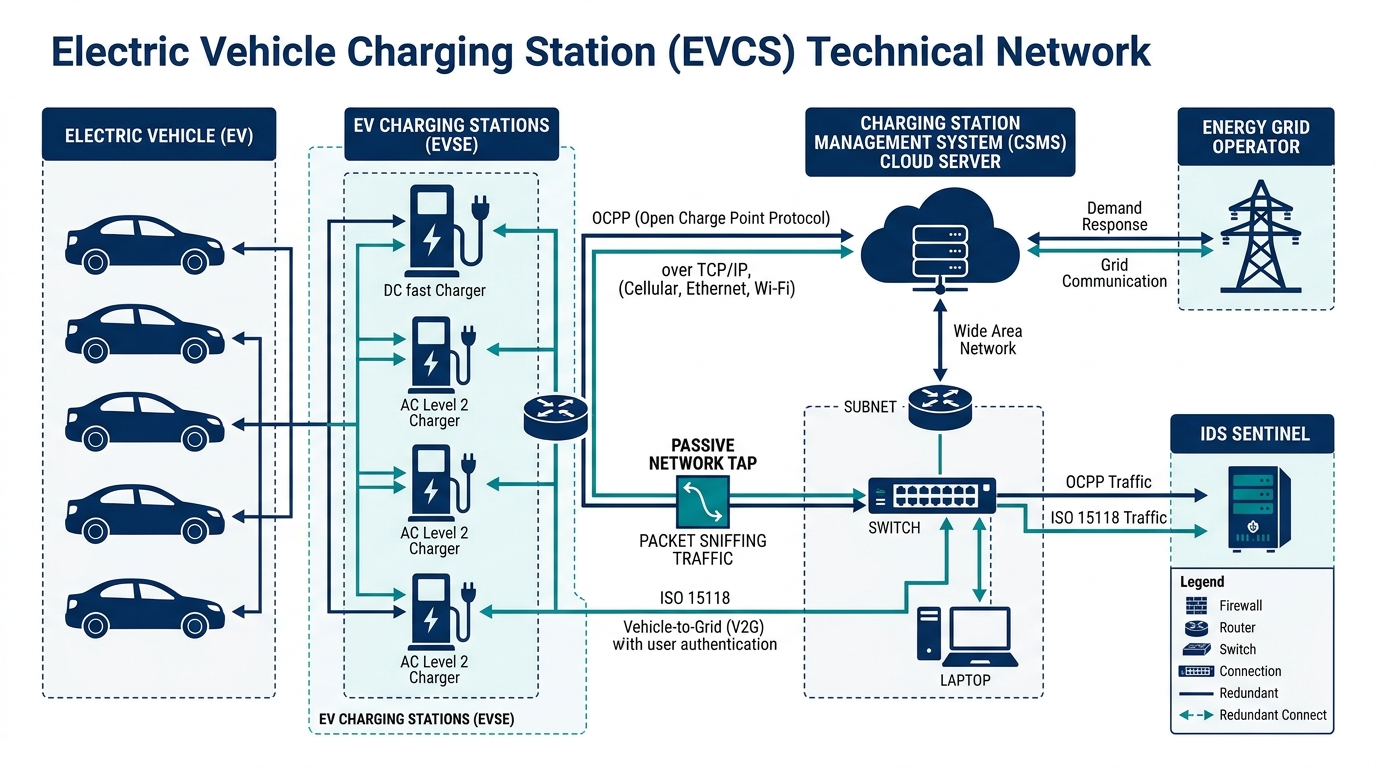
\includegraphics[width=0.92\textwidth]{images/evcs-network-topology.jpg}
    \caption{EVCS technical network architecture showing chargers (EVSE), CSMS cloud server, power grid communication, and the passive network tap monitoring point where flow data is captured.}
    \label{fig:network_topology}
\end{figure}

\subsection{Network Monitoring Point}

The CICEVSE2024 dataset was generated by placing a passive network tap at the aggregation switch connecting multiple EVSE units to the CSMS. All traffic—benign transactions, firmware exchanges, and injected attack flows—was captured as full PCAP files and subsequently converted to \textit{flow-level} records using CICFlowMeter, yielding 83 bidirectional features per flow.

% ============================================================================
% 3. DATASET & NETWORK TRAFFIC ANALYSIS
% ============================================================================
\section{CICEVSE2024: Network Traffic Dataset}

\subsection{Dataset Composition}

The CICEVSE2024 dataset, published by the Canadian Institute for Cybersecurity (University of New Brunswick), contains $\sim$1.92 million bidirectional network flows across 15 classes (1 Benign + 14 attack types).

\begin{table}[H]
\centering
\caption{CICEVSE2024 Traffic Class Distribution}
\begin{tabular}{|l|r|l|}
    \hline
    \textbf{Traffic Class} & \textbf{Flows} & \textbf{Category} \\ \hline
    Benign & 209,987 & Normal \\ \hline
    DoS SlowHTTPTest & 415,821 & Denial of Service \\ \hline
    DoS Slowloris & 202,461 & Denial of Service \\ \hline
    DoS GoldenEye & 58,391 & Denial of Service \\ \hline
    DoS Hulk & 130,207 & Denial of Service \\ \hline
    DDoS LOIC-HTTP & 73,108 & Distributed DoS \\ \hline
    DDoS HOIC & 56,992 & Distributed DoS \\ \hline
    Nmap OS Scan & 48,721 & Reconnaissance \\ \hline
    Nmap TCP Scan & 89,134 & Reconnaissance \\ \hline
    Nmap UDP Scan & 61,222 & Reconnaissance \\ \hline
    \multicolumn{3}{|l|}{\textit{+ 4 additional attack classes (FTP Patator, SSH Patator, etc.)}} \\ \hline
    \textbf{Total} & \textbf{$\sim$1.92M} & \textbf{15 classes} \\ \hline
\end{tabular}
\end{table}

\subsection{Key Network Flow Features}

Each flow record contains 83 features extracted by CICFlowMeter. The most discriminative (after leakage removal) include:

\begin{table}[H]
\centering
\caption{Critical Network Flow Features for Intrusion Detection}
\begin{tabular}{|l|p{8cm}|}
    \hline
    \textbf{Feature} & \textbf{Network Significance} \\ \hline
    \texttt{dst\_port} & Destination port; directly identifies port scan targets (dropped by the reference pipeline—a critical error) \\ \hline
    \texttt{bidirectional\_packets} & Total packets in the flow; high counts signal flood attacks \\ \hline
    \texttt{bidirectional\_bytes} & Total bytes; volumetric signature of DoS \\ \hline
    \texttt{bidirectional\_duration\_ms} & Flow duration; Slowloris keeps connections alive far longer than benign OCPP \\ \hline
    \texttt{src2dst\_mean\_ps} & Mean packet size source→destination; large payloads vs.\ probing SYN packets \\ \hline
    \texttt{dst2src\_packets} & Reverse-direction packets; absent in half-open scans, high in established connections \\ \hline
    \texttt{src\_port} & Ephemeral source port; bands per capture session (partial fingerprint) \\ \hline
\end{tabular}
\end{table}

\begin{figure}[H]
    \centering
    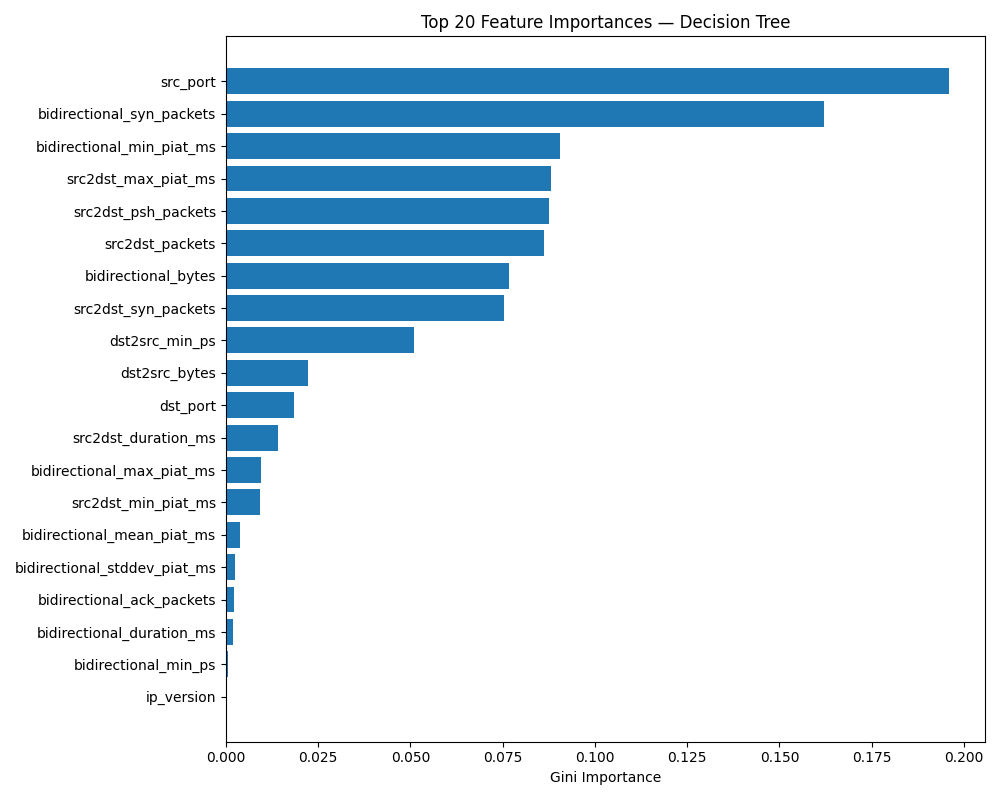
\includegraphics[width=0.85\textwidth]{images/feature-importance.png}
    \caption{Top discriminative network flow features from the corrected leak-free model after removing timestamp epoch identifiers.}
    \label{fig:feature_importance}
\end{figure}

% ============================================================================
% 4. NETWORK ATTACK TAXONOMY
% ============================================================================
\section{Network Attack Taxonomy in EVCS}

The attacks present in CICEVSE2024 map directly to well-known network attack categories:

\subsection{Denial-of-Service (DoS / DDoS)}

\begin{itemize}[leftmargin=1.4em, itemsep=0.2em]
    \item \textbf{Volumetric Floods} (Hulk, GoldenEye, LOIC-HTTP, HOIC): Overwhelm the EVCS with high packet/byte rates, disrupting charging session management and OCPP communication.
    \item \textbf{Slow-rate Attacks} (Slowloris, SlowHTTPTest): Exhaust server connection pools by holding HTTP connections open with minimal traffic—difficult to detect by volume alone; identifiable by anomalous \texttt{bidirectional\_duration\_ms}.
\end{itemize}

\begin{resultbox}[title={\textbf{Detection Result — DoS}}]
    All flood-type attacks achieve \textbf{F1 $\geq$ 0.999} with the corrected pipeline. Slow-rate attacks are also well-detected due to distinctive flow-duration signatures.
\end{resultbox}

\subsection{Reconnaissance (Network Scanning)}

\begin{itemize}[leftmargin=1.4em, itemsep=0.2em]
    \item \textbf{Nmap TCP/UDP/OS Scans:} Probe open ports and services on EVCS endpoints. These generate many short-lived flows with varied \texttt{dst\_port} values.
    \item \textbf{The \texttt{dst\_port} problem:} The reference pipeline \textit{drops} \texttt{dst\_port}—the single feature that \textit{defines} a port scan—making scan classification nearly impossible from remaining features alone.
\end{itemize}

\begin{findingbox}[title={\textbf{Detection Result — Reconnaissance}}]
    Scan-type attacks achieve only \textbf{F1 0.10--0.27} after leakage correction. Mutual information analysis shows the best remaining feature explains only \textbf{5\%} of scan-type variance—the detection ceiling is a \textit{data limitation}, not a model limitation.
\end{findingbox}

\subsection{Brute-Force \& Application-Layer Attacks}

FTP Patator and SSH Patator attacks target authentication services on the EVCS management interface. These produce many failed-login flows with characteristic packet sizes and connection-reset patterns.

\begin{figure}[H]
    \centering
    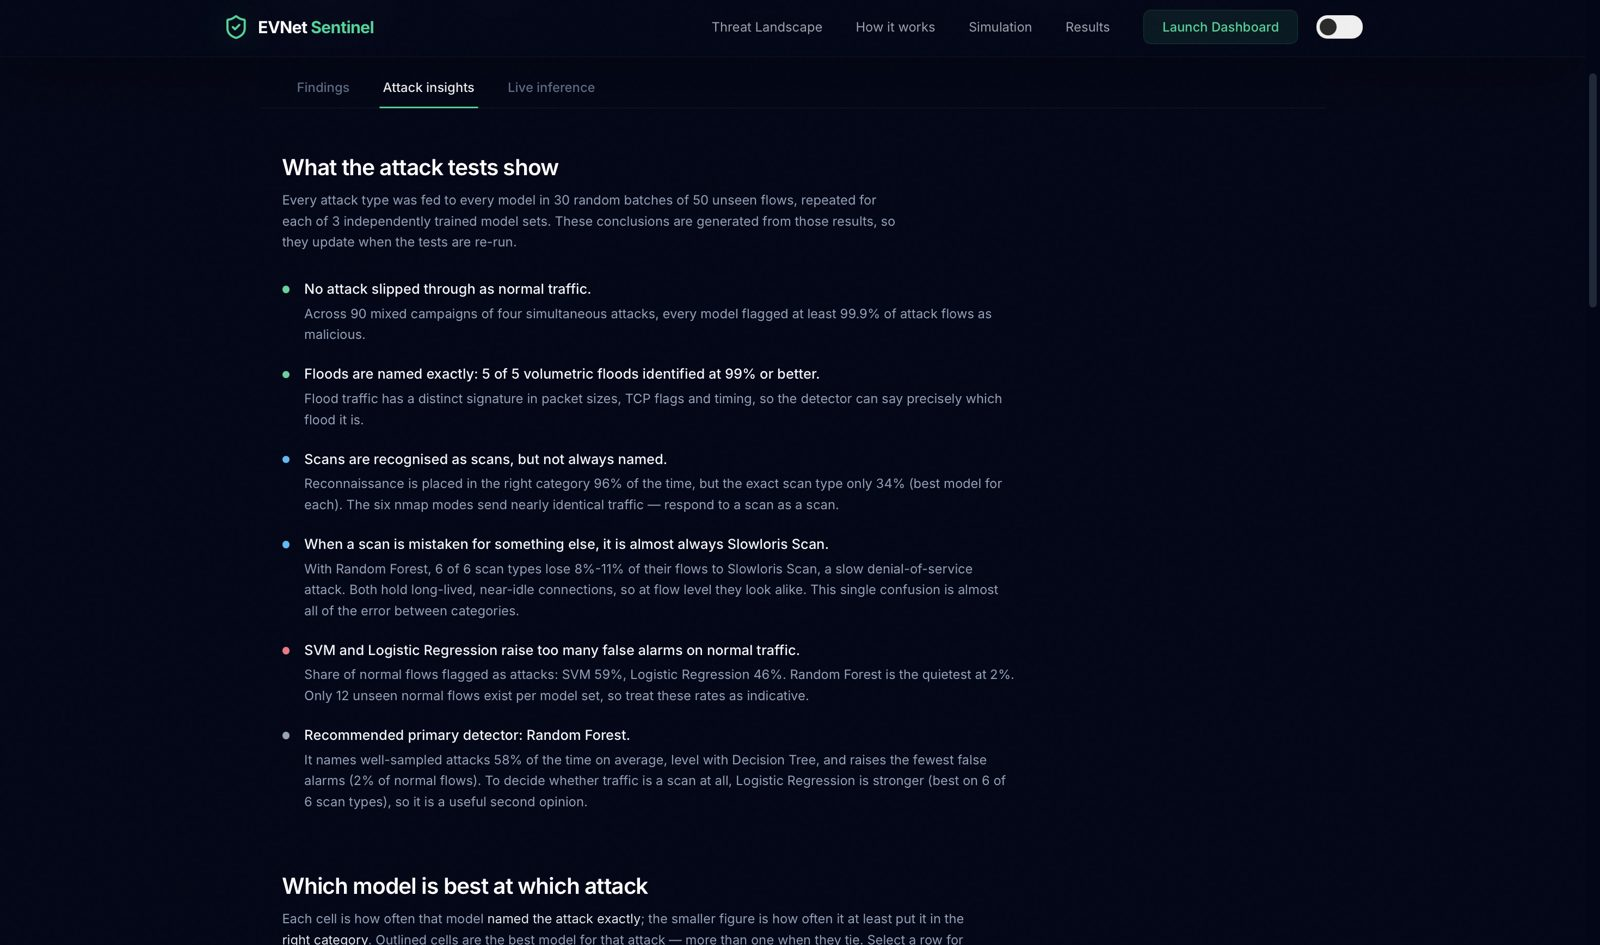
\includegraphics[width=0.90\textwidth]{images/attack-insights.jpg}
    \caption{The ``Attack Insights'' console in EVNet Sentinel showing per-attack empirical performance, false alarm rates, and operator response instructions.}
    \label{fig:attack_insights}
\end{figure}

% ============================================================================
% 5. DATA LEAKAGE: A NETWORK-LEVEL EXPLANATION
% ============================================================================
\section{Data Leakage Audit: Network-Level Findings}

The central contribution of EVNet Sentinel is identifying that the published 98.4\% accuracy was inflated by non-network-behavioral features leaking capture metadata. All five findings have a network-level explanation:

\begin{findingbox}[title={\textbf{Finding 1 — Timestamp Leak}}]
    Each attack type was recorded in a separate PCAP file at a distinct wall-clock time. The six \texttt{*\_first\_seen\_ms} / \texttt{*\_last\_seen\_ms} columns encode \textit{when the capture was taken}, not any property of the network flow itself. A single Decision Tree on \texttt{bidirectional\_first\_seen\_ms} alone scores \textbf{0.9976} accuracy—above the published 0.9840.
\end{findingbox}

\begin{findingbox}[title={\textbf{Finding 2 — \texttt{dst\_port} Dropped}}]
    The reference pipeline removes \texttt{dst\_port} (the destination port number), the feature that \textit{defines} a port scan at the network level, while retaining the leaky timestamps.
\end{findingbox}

\begin{findingbox}[title={\textbf{Finding 3 — Stream Ordering}}]
    In original capture order, the attack label changes only 54 times across 1.92M flows. A trivial ``repeat the last label'' rule scores \textbf{0.99997}—any sequential model (including ARF + ADWIN) benefits from this temporal autocorrelation, not from learning network patterns.
\end{findingbox}

\begin{findingbox}[title={\textbf{Finding 4 — Drift Alarms = File Seams}}]
    42 of 43 ADWIN drift alarms fall within 100 flows of a join between PCAP files ($p < 0.0005$). The drift detector responded to \textit{file concatenation boundaries}, not genuine concept drift in network traffic.
\end{findingbox}

\begin{findingbox}[title={\textbf{Finding 5 — \texttt{src\_port} Fingerprint}}]
    Ephemeral source ports band per capture session. \texttt{src\_port} acts as a partial session identifier rather than a behavioral network feature. Removing it costs Decision Tree twice the performance it costs Random Forest.
\end{findingbox}

\begin{figure}[H]
    \centering
    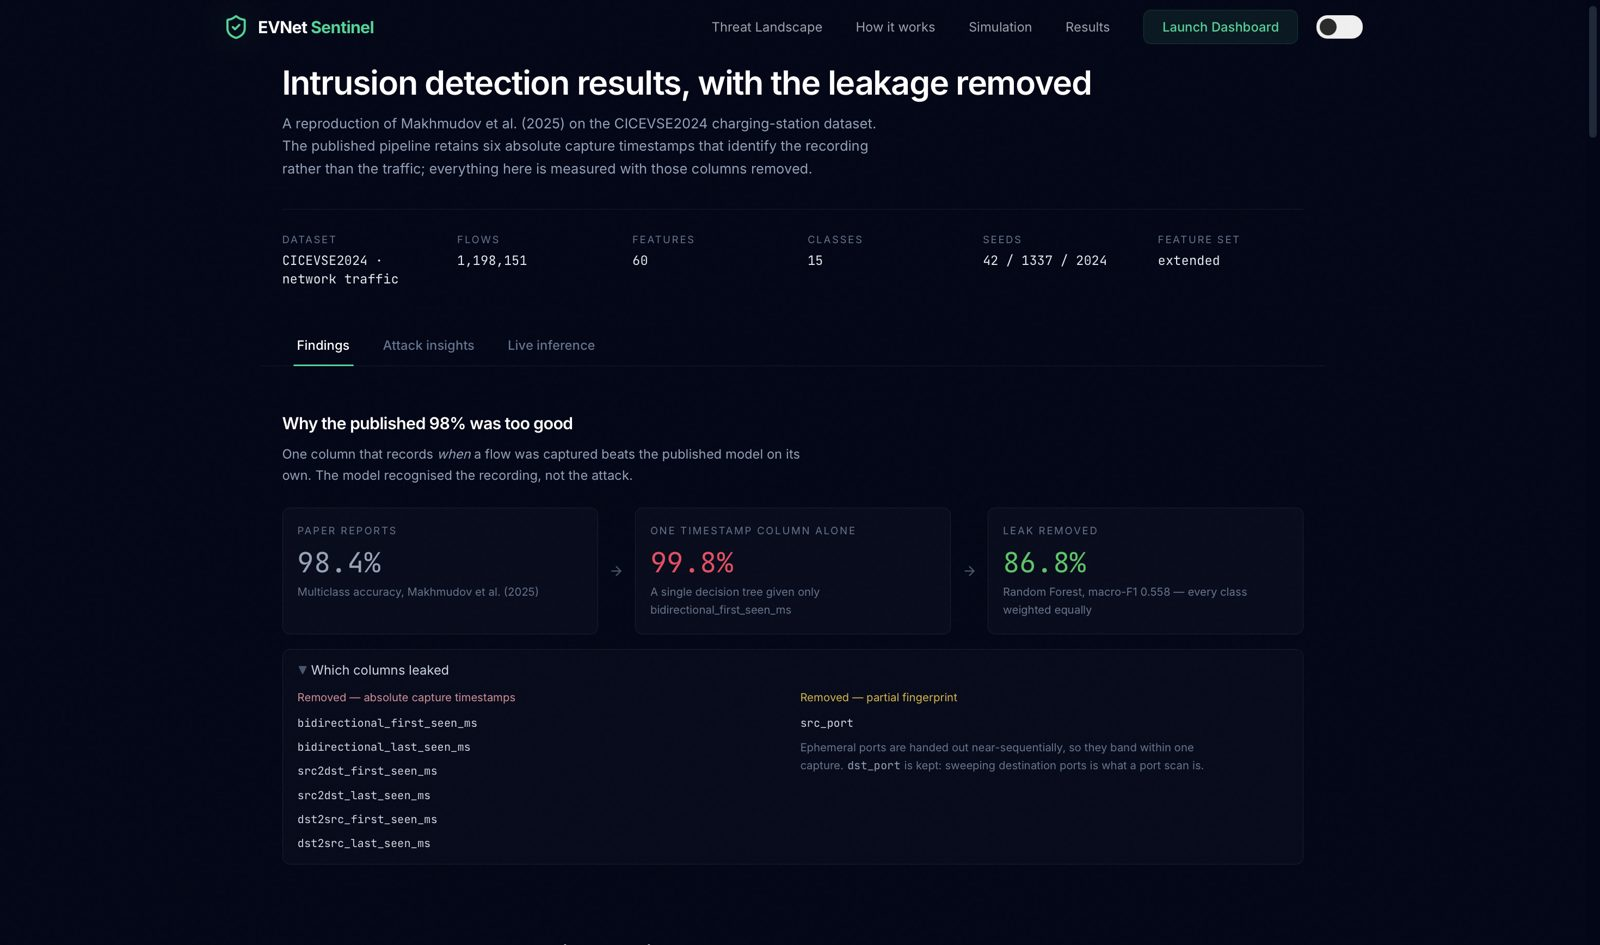
\includegraphics[width=0.90\textwidth]{images/dashboard.jpg}
    \caption{The ``Findings'' dashboard highlighting the audit evidence: timestamp-only classification (99.76\%), capture-order autocorrelation (99.99\%), and true corrected macro-F1 (0.558).}
    \label{fig:leakage_dashboard}
\end{figure}

% ============================================================================
% 6. CORRECTED IDS METHODOLOGY
% ============================================================================
\section{Corrected Intrusion Detection Methodology}

\subsection{Leak-Free Preprocessing Pipeline}

The corrected pipeline applies the following network-aware transformations:

\begin{enumerate}[leftmargin=1.6em, itemsep=0.3em]
    \item \textbf{Drop timestamp columns:} All six \texttt{*\_first\_seen\_ms} / \texttt{*\_last\_seen\_ms} epoch columns removed.
    \item \textbf{Retain \texttt{dst\_port}:} The destination port is a legitimate network feature essential for scan detection.
    \item \textbf{Shuffle before split:} Destroy capture-order autocorrelation; perform stratified 80/20 train/test split.
    \item \textbf{Deduplicate:} Remove exact-duplicate flow rows (an artefact of CICFlowMeter window overlap).
    \item \textbf{StandardScaler:} Fit on training set only to prevent test-set information leakage.
\end{enumerate}

\subsection{Model Benchmarking}

Six classifiers were evaluated on the corrected, leak-free dataset across 3 random seeds:

\begin{table}[H]
\centering
\caption{Corrected Model Benchmark Results (Leak-Free, 3-Seed Average)}
\begin{tabular}{|l|c|c|c|l|}
    \hline
    \textbf{Model} & \textbf{Macro-F1} & \textbf{Accuracy} & \textbf{False Alarms} & \textbf{Notes} \\ \hline
    \textbf{Random Forest} & \textbf{0.558 $\pm$ 0.008} & 0.868 & 3\% & Highest macro-F1 \\ \hline
    Decision Tree & 0.557 $\pm$ 0.010 & 0.868 & 11\% & \\ \hline
    XGBoost & 0.551 $\pm$ 0.011 & 0.869 & 2\% & \textbf{Recommended} (fewest false alarms) \\ \hline
    LightGBM & 0.550 $\pm$ 0.004 & 0.868 & 3\% & \\ \hline
    Logistic Regression & 0.436 $\pm$ 0.017 & 0.863 & 44\% & Best on scans \\ \hline
    SVM & 0.411 $\pm$ 0.017 & 0.862 & 58\% & \\ \hline
\end{tabular}
\end{table}

\noindent
\textit{Key observation:} All four tree-based models are statistically tied at $\sim$0.55 macro-F1. The accuracy of $\sim$0.87 is driven by the dominant flood classes; \textbf{macro-F1} is the correct headline metric because it equally weights all 15 classes, including the poorly-detected scans.

\begin{figure}[H]
    \centering
    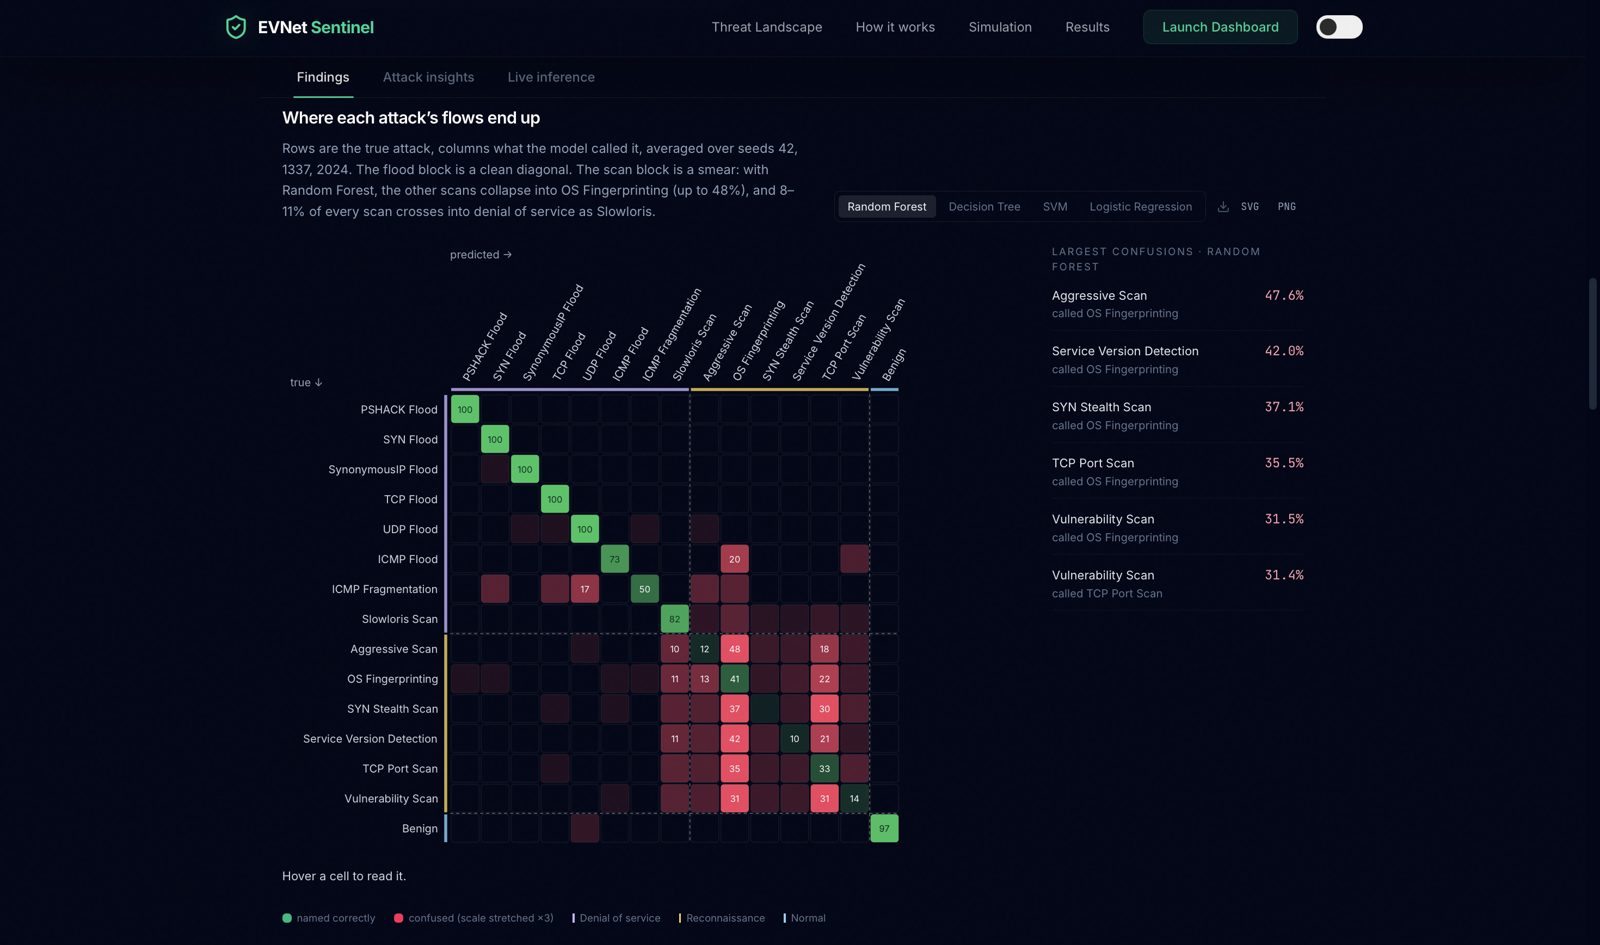
\includegraphics[width=0.90\textwidth]{images/confusion-matrix.jpg}
    \caption{Interactive multi-class confusion matrix explorer showing sharp diagonal concentration for volumetric floods alongside horizontal dispersion across scan variants.}
    \label{fig:confusion_matrix}
\end{figure}

% ============================================================================
% 7. CLOSED-LOOP NETWORK RESPONSE
% ============================================================================
\section{Closed-Loop Network Response System}

Beyond detection, EVNet Sentinel implements a closed-loop containment policy modeled on real network defense practices:

\begin{table}[H]
\centering
\caption{Threat Level Escalation and Network Response Actions}
\begin{tabular}{|l|l|p{7cm}|}
    \hline
    \textbf{Threat Level} & \textbf{Trigger} & \textbf{Network Response} \\ \hline
    \textcolor{accent}{\textbf{Safe}} & No malicious flows & Normal EVCS operation \\ \hline
    \textcolor{warning}{\textbf{Elevated}} & Scan detected & Restrict scanning IP; rate-limit connections \\ \hline
    \textcolor{danger}{\textbf{Not Safe}} & Flood / DDoS detected & Quarantine attacker IP at firewall; terminate malicious sessions \\ \hline
\end{tabular}
\end{table}

\noindent
The response system was replayed over all 20 recorded attacker--attack pairs in the dataset. A scanner that later escalates to flooding is automatically quarantined on its first flood flow—demonstrating adaptive, stateful network defense.

\begin{figure}[H]
    \centering
    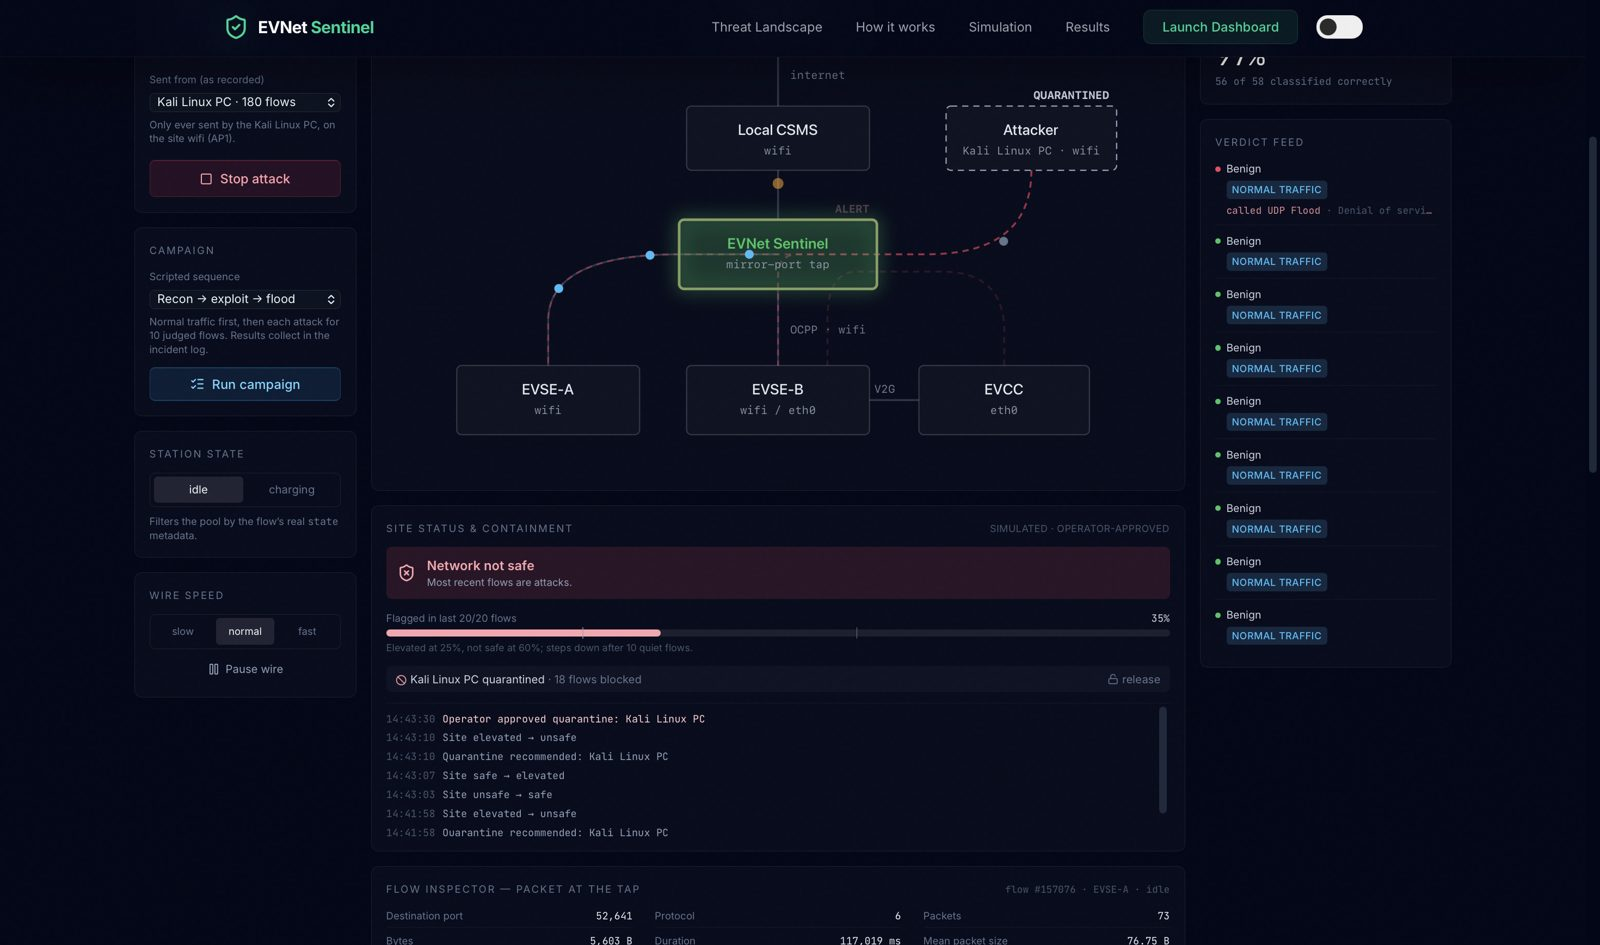
\includegraphics[width=0.90\textwidth]{images/simulation-quarantine.jpg}
    \caption{Interactive simulation console demonstrating state transition to ``Network Not Safe'' with closed-loop operator containment quarantine triggered on malicious traffic.}
    \label{fig:simulation_quarantine}
\end{figure}

% ============================================================================
% 8. SYSTEM ARCHITECTURE (NETWORK VIEW)
% ============================================================================
\section{System Architecture — Network Perspective}

The EVNet Sentinel deployment uses a decoupled client-server architecture:

\begin{highlightbox}[title={\textbf{Network Communication}}]
\begin{itemize}[leftmargin=1.2em, itemsep=0.2em]
    \item \textbf{FastAPI Backend} (\texttt{:8000}): Serves REST endpoints (\texttt{POST /predict}) for single-flow classification. Loads trained models from \texttt{saved\_models/} at startup via a dynamic model registry.
    \item \textbf{Next.js Frontend} (\texttt{:3100}): Reads pre-exported JSON results from \texttt{frontend/data/} — no runtime API dependency, enabling deployment on a fresh clone without the dataset.
    \item \textbf{WebSocket Channel}: Real-time push of predictions and threat-level changes from backend to dashboard.
    \item \textbf{Docker Containerization}: Single-stage build preserving Rust/C++ compilation artefacts required by the \texttt{river} streaming ML library.
\end{itemize}
\end{highlightbox}

\begin{figure}[H]
    \centering
    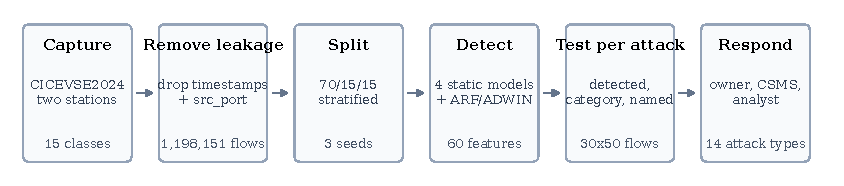
\includegraphics[width=0.92\textwidth]{figures/fig_pipeline.pdf}
    \caption{Comprehensive end-to-end system and ML pipeline architecture spanning CICEVSE2024 ingestion, leak-free training, dynamic FastAPI model registry, and Next.js presentation.}
    \label{fig:architecture_pipeline}
\end{figure}

% ============================================================================
% 9. CONCLUSION
% ============================================================================
\section{Conclusion}

This project demonstrates the critical importance of \textbf{network-aware feature engineering} in building reliable intrusion detection systems. The five leakage findings show that high-accuracy claims can arise from capture metadata rather than genuine network behavior. After correction:

\begin{itemize}[leftmargin=1.4em, itemsep=0.3em]
    \item \textbf{Flood attacks} (DoS/DDoS) are near-perfectly detectable (F1 $\geq$ 0.999) from volumetric flow features.
    \item \textbf{Reconnaissance scans} remain a hard problem (F1 0.10--0.27) due to data-level limitations—the single best feature explains only 5\% of scan-type variance.
    \item The \textbf{corrected macro-F1 of 0.558 $\pm$ 0.008} is the honest baseline for future EVCS network security research on this dataset.
    \item A \textbf{closed-loop response system} demonstrates how detection feeds into practical network containment (quarantine, restriction, session termination).
\end{itemize}

\noindent
Future work includes deploying the IDS on live OCPP traffic streams, incorporating deep-packet inspection for encrypted V2G payloads, and investigating graph-neural-network approaches for modeling station-to-station communication patterns.

% ============================================================================
% REFERENCES
% ============================================================================
\section*{References}
\addcontentsline{toc}{section}{References}

\begin{enumerate}[leftmargin=1.6em, itemsep=0.3em, label={[\arabic*]}]
    \item F.~Makhmudov, D.~Kilichev, U.~Giyosov, F.~Akhmedov, ``Online Machine Learning for Intrusion Detection in Electric Vehicle Charging Systems,'' \textit{Mathematics}, vol.~13, no.~5, p.~712, 2025.

    \item E.~D.~Buedi, A.~A.~Ghorbani, S.~Dadkhah, R.~L.~Ferreira, ``Enhancing EV Charging Station Security Using a Multi-dimensional Dataset: CICEVSE2024,'' in \textit{Data and Applications Security and Privacy XXXVIII (DBSec 2024)}, LNCS vol.~14901, Springer, 2024, pp.~171--190.

    \item C.~Joglekar, C.~Eze, D.~Xiang, A.~Monti, ``A Hybrid Intrusion Detection System for Electric Vehicle Charging Infrastructure,'' \textit{arXiv:2606.23236}, 2026.

    \item J.~Bean, D.~M.~Manias, ``Cybersecurity of Electric Vehicle Charging Infrastructure: Recent Advances, Open Challenges, and Future Directions,'' \textit{arXiv:2605.24190}, 2026.

    \item A.~Dridi, C.~Gamboa, M.~Elrawy, \textit{et al.}, ``A Survey on Cybersecurity of Autonomous and Connected Electric Vehicles,'' \textit{IEEE Access}, vol.~12, pp.~1--24, 2024.

    \item Open Charge Alliance, ``OCPP 2.0.1 Specification,'' \url{https://www.openchargealliance.org/}, 2022.

    \item ISO, ``ISO 15118:2019 — Road vehicles — Vehicle to grid communication interface,'' International Organization for Standardization, 2019.

    \item TATU-hacker, ``Intrusion Detection on Electric Vehicle Charging Systems,'' GitHub Repository, \url{https://github.com/TATU-hacker/Intrusion_Detection_on_Electric_Vehicle_Charging_Systems}.
\end{enumerate}

\end{document}
